\documentclass[titlepage]{jarticle}
\usepackage{abstract}
\usepackage[dvipdfmx]{graphicx}
\usepackage{amsmath}
\usepackage{ascmac}
\usepackage{caption}
\usepackage{url}

\title{新規暗号の提案及び安全性評価}
\author{石川琉聖\\立命館大学 情報理工学部}
\date{\today}

\begin{document}

\maketitle

\begin{abstract}
本論文では, 新たな現代暗号かつ転置式暗号としてcubing暗号を提案する.cubing暗号はルービックキューブの転置を参考にし,任意の平文を転置する.しかし,cubing暗号は平文長が45Byteで定義されているため,45Byte以上の平文は暗号化できない.そこで,本論文では新たな暗号利用モードであるcubingmodeを提案する.cubingmodeは平文長を可変にするだけでなく,暗号文ブロックがすり替えられないようブロック間をシャッフルする機能や,頻度分析ができなくなるよう平文を乱数化する処理を行った.また,cubingmodeを利用した際のcubing暗号の安全性評価を行った.その結果,一般的な暗号の攻撃手法では解読できないことがわかった.だが,cubing暗号はアルゴリズムによって出力されるデータが大きいことや,暗号化に時間がかかるといった問題点もみられた.
\end{abstract}

\tableofcontents
\newpage

\section{はじめに}
\subsection{背景}
インターネットの普及により,研究機関のみならず個人もインターネットを使うようになった.それに伴い,個人情報や社外秘情報などがインターネット上で取引され,情報の秘匿性が重要視されるようになった.それら秘匿情報を第三者に見られないようにするため,インターネット上では暗号技術というものが使われている.暗号技術とは特定の情報を隠蔽する技術で,その代表的なものにシーザー暗号やエニグマ暗号などがある.現在頻繁に使われる暗号としてRSA暗号やAES暗号があり,インターネット上で殆ど全ての秘匿情報を扱う際に利用されている.\\

\subsection{Our Contribution}
本論文では新しい暗号cubing暗号を提案する.現代暗号の多くは換字式暗号であり,転置式暗号は数少ない.だが,cubing暗号のアルゴリズムは現代暗号でありつつ転置式暗号である.cubing暗号はルービックキューブに着想を得た転置を行う.また,cubing暗号での利用を想定とした暗号利用モードであるcubingmodeも提案する.\\
さらに,cubing暗号をcubingmodeで利用した際の安全性の評価を行った.本論文では,適切な鍵長の計算,ブルートフォース攻撃対策,頻度分析,選択平文攻撃,replay攻撃について分析した.分析の結果,鍵長は\(50\)文字\(=50\text{Byte}\)以上が良く,いずれの攻撃手法においてもcubing暗号に対しては有効ではないことがわかった.

\subsection{定義}
\subsubsection{ルービックキューブ}
ルービックキューブとは,ハンガリーの建築学者ルビク・エルネーが考案した立体パズルである.一般的なルービックキューブは\(3\times 3\times 3=9\)個の正方形のキューブからなり,6つの各面には色がついている.これらのキューブを、各行または列ごとに自由に回転させることができる。このパズルは,回転操作によってシャッフルされた状態のルービックキューブを元の配置に戻すことを目標として遊ぶ.\\

\begin{figure}
  \centering
  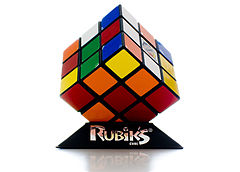
\includegraphics[width=10cm]{./tex_pic/rubik-cube.jpg}\\
  \caption{ルービックキューブ\\(https://ja.wikipedia.org)}
\end{figure}

\subsubsection{列によるルービックキューブの表現}
ルービックキューブをコンピュータ上で表現する際には列を用いる.具体的には以下のルービックキューブの展開図とコンピュータ上で扱う列が対応する.また,列の各要素をマスと呼び,文字\(C\)が列内の\(i\)番目にある場合,列番号は\(i\)とする..\\
\begin{center}
  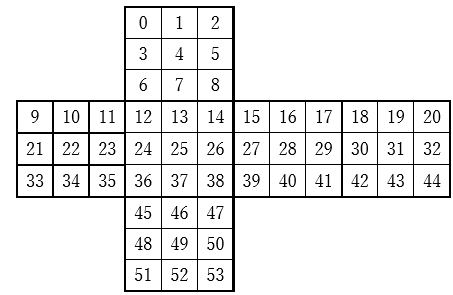
\includegraphics[width=7cm]{./tex_pic/seq.jpg}\\
\end{center}

\subsubsection{表示可能文字}
文字Xが表示可能文字であるとは,付録1に定義された列printable\_tableにXが含まれていることを指す.エスケープシーケンスに関してはASCIIコードに準じている.

\subsubsection{62進数}
62進数とは,62を底とした位取り記数法における数である.付録2に定義されたアルファベットの大小と数字列からなる.具体的な順序は付録2に記した.例えば,10進数の0は62進数のAであり,10進数の1は62進数のBである.また,10進数の\(62^2-1\)は62進数の99である.

\subsubsection{鍵}
鍵は,同じ暗号方式を使用しながら利用者毎に暗号化の手順を異なるものにするために使用される。cubing暗号の鍵は\(3n\)文字\((n=1,2,...)\)であり,'1','2','3'の三種類の文字で構成される.

\subsubsection{暗号利用モード}
暗号利用モードとは,暗号化アルゴリズムで定義された平文長よりも長い平文を暗号化するためのアルゴリズムのことである.暗号利用モードではブロックと呼ばれる,複数の文字からなる特定の長さの列ごとに暗号化を行う,

\subsubsection{ECBモード}
ECBモードは暗号利用モードの一種で,全てのブロックを同じ鍵で暗号化し,最後に暗号化されたブロックを結合するアルゴリズムである.これにより,二種類の鍵(\(K_i,K_j\))と二種類の平文ブロック(\(P_i,P_j\))があり,鍵Kと平文ブロックPで生成される暗号文ブロックを\(C(K,P)\)とし,\(K_i=K_j\)かつ\(P_i=P_j\)である時,必ず\(C(K_i,P_i)=C(K_j,P_j)\)となる.

\section{cubing暗号}
\subsection{cubing暗号の概要}
cubing暗号は平文ブロック長45Byte,暗号文ブロック長54Byte,鍵長可変の転置式暗号である.この暗号は暗号化及び復号の並列化が可能であるが,暗号化の場合は後に説明するShuffle処理,復号の場合はSort処理が並列化できないのでボトルネックとなる.なお,本暗号に関するソースコードは公開した.\footnote{https://github.com/xryuseix/cubing\_cipher/blob/master/cubing.cpp}

\subsection{cubing暗号の暗号化・復号手順}
暗号化及び復号では以下の処理を利用する.

\subsubsection{パディング処理}
平文ブロックが45Byteに満たない場合,1Byte分のnull\footnote{nullは「何も示さないもの」を表す}入れ,残りはランダムな英数列を入れる.これにより,平文を45Byteに固定することができる.

\subsubsection{転置の仕様}
cubing暗号の転置は方向・列・回数の三つより決定される.鍵の左から\(3n+1\)文字目が方向,\(3n+2\)文字目が列,\(3n+3\)文字目が回数を表す\((n=0,1,2,...)\).方向に関しては以下の図のように三種類定義される.なお,図には各方向に対する列が記載されている.画像は全て\url{http://iamthecu.be/}にて作成した.

\begin{figure}[htb]
  \centering
  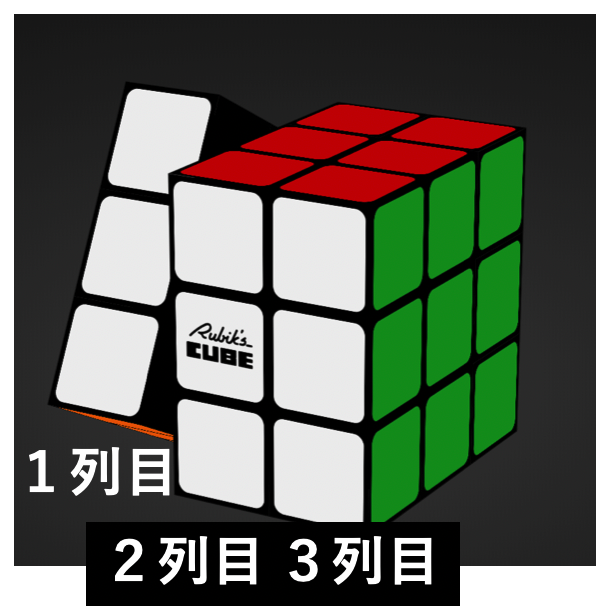
\includegraphics[width=5cm]{./tex_pic/tate.jpg}
  \caption{1列目を縦方向に回転させたとき}
\end{figure}
\begin{figure}[htb]
  \centering
  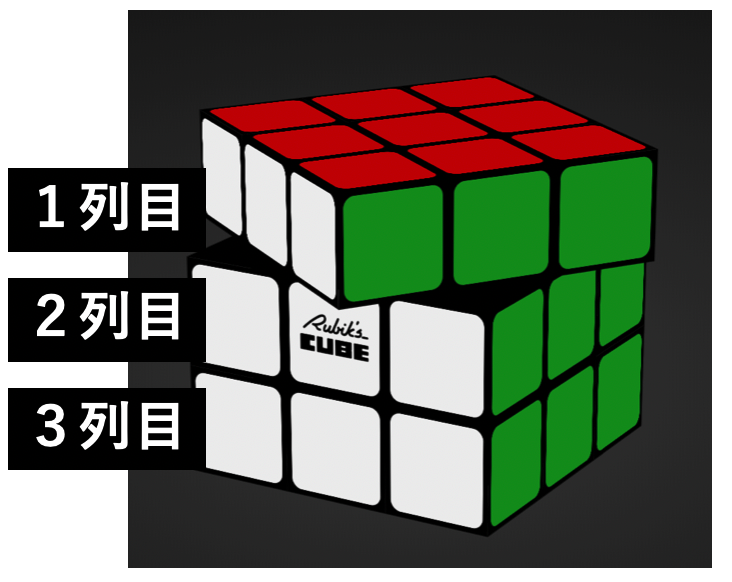
\includegraphics[width=5cm]{./tex_pic/yoko.jpg}
  \caption{1列目を横方向に回転させたとき}
\end{figure}
\begin{figure}[!h]
  \centering
  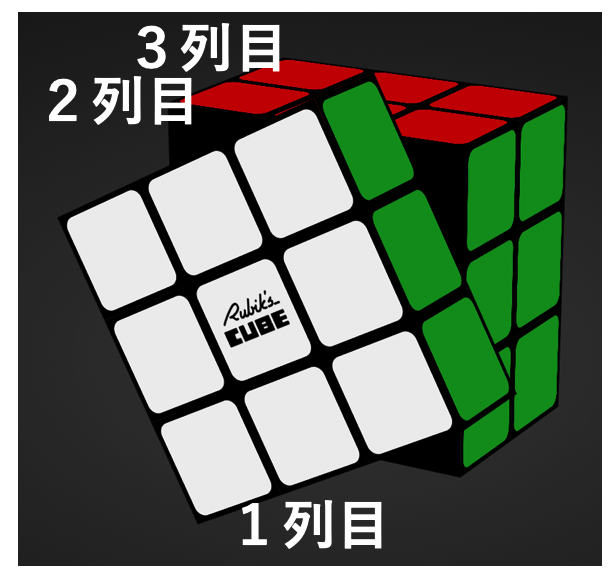
\includegraphics[width=5cm]{./tex_pic/kai.jpg}
  \caption{1列目を回転方向に回転させたとき}
\end{figure}

なお,cubing暗号の転置はルービックキューブの転置と比較して,「ある方向のある列を転置させる際,他の列およびマスは一切転置させない」という点において異なる.具体的には以下の図のような転置がなされる.\\
\begin{center}
  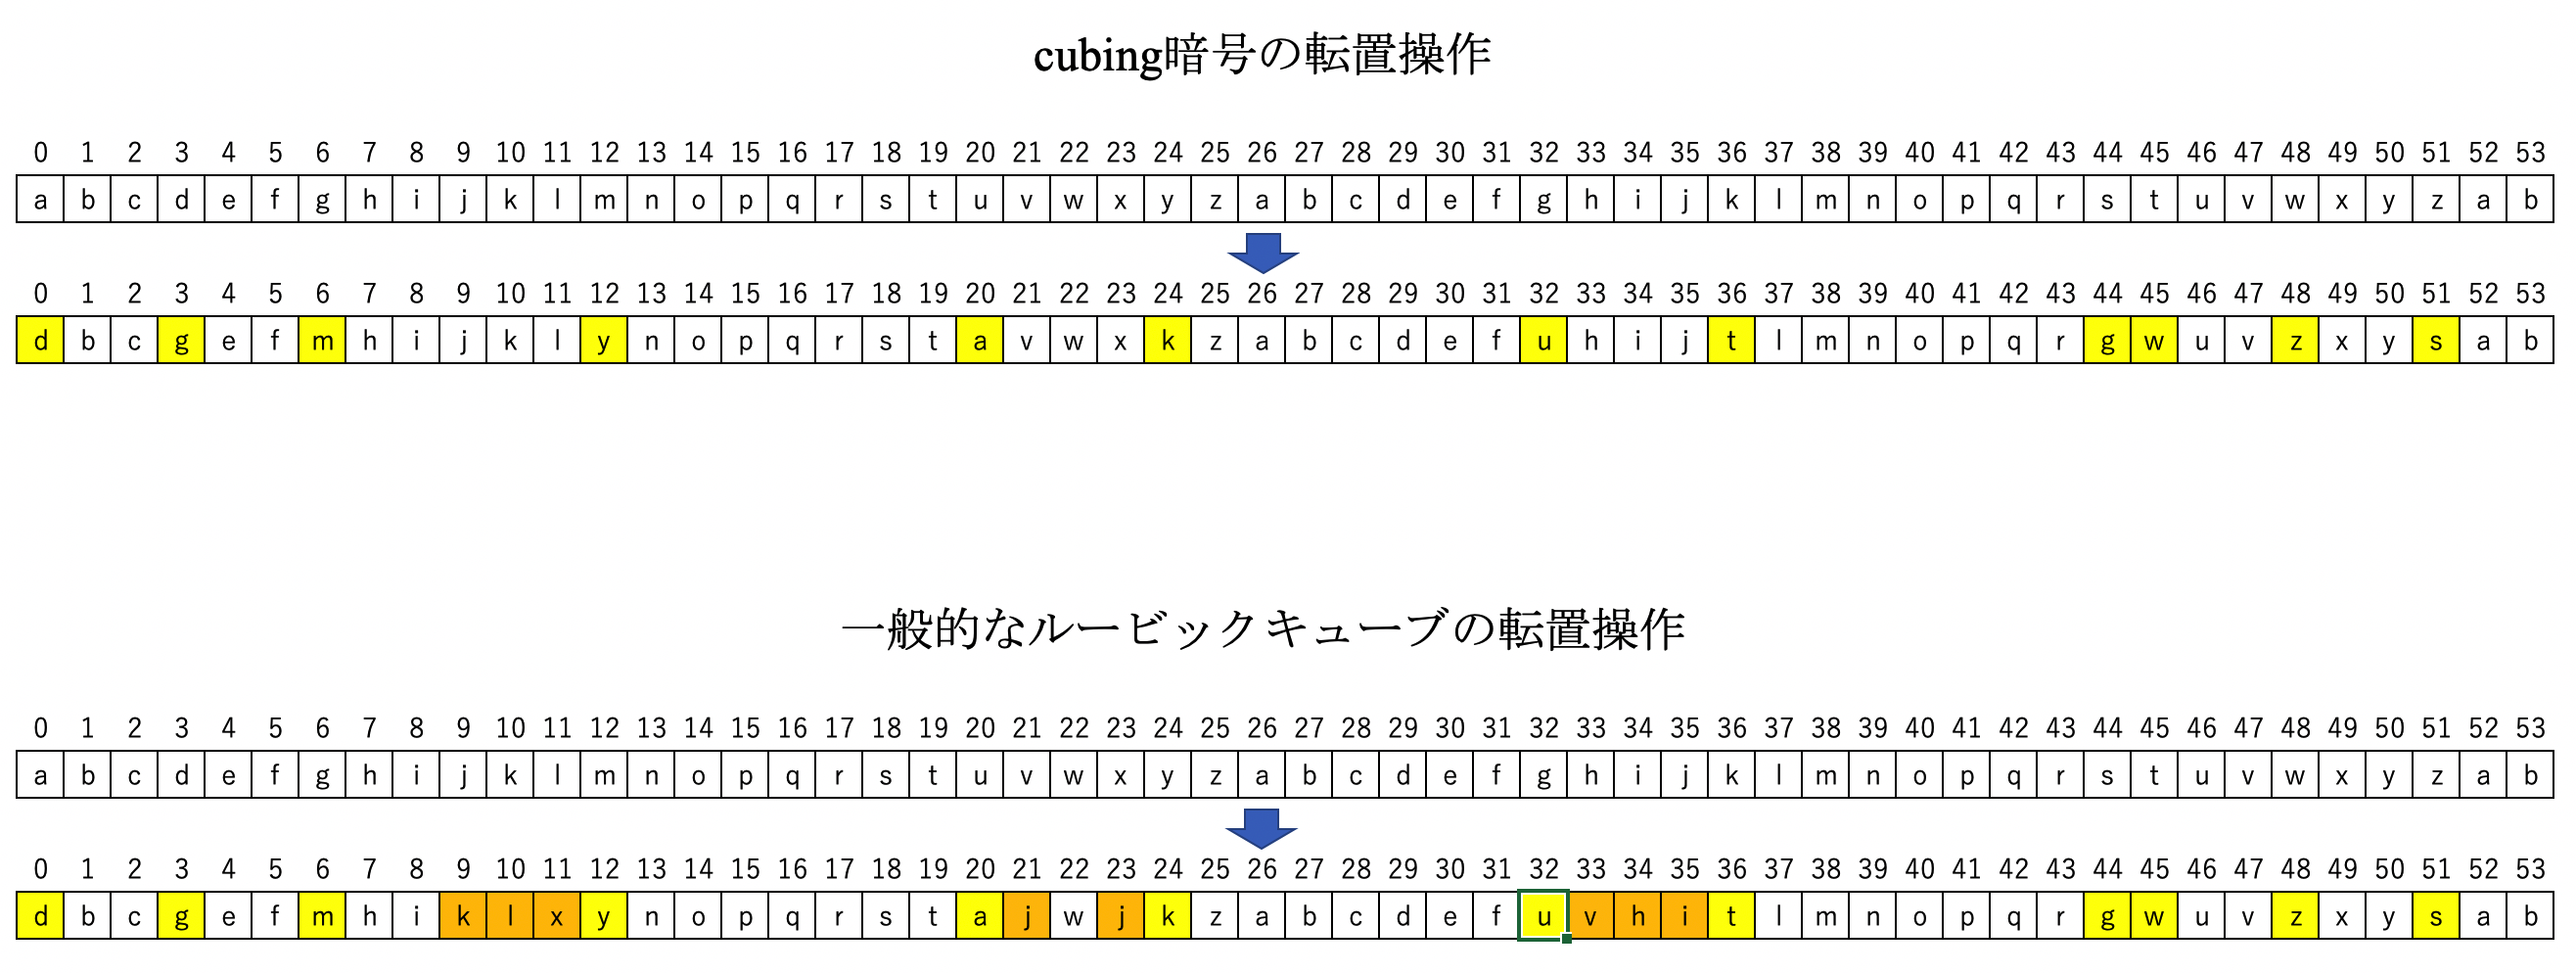
\includegraphics[width=12cm]{./tex_pic/trans.png}\\
\end{center}
本節では,「鍵とは縦方向1列1回の回転を表すもの」とする.まず「cubing暗号の転置操作」の黄色のマスは鍵の転置操作で場所が入れ替わったマスを表している.一方,「一般的なルービックキューブの転置操作」の黄色のマスは同じ鍵で「cubing暗号の転置操作」に加えてさらに場所が入れ替わるマスである.一見一回の操作で多くの列を転置できるように見えるが,実際はルービックキューブの角の3列や,側面の2列は常に隣り合った関係を持ってしまう.よって全探索や頻度分析の手掛かりになってしまうと考えた.したがって,このような転置はしないようにした.

また,以下の順序で暗号化及び復号を行う.
\subsubsection{暗号化}
\begin{enumerate}
\item 平文を用意する.
\item パディング処理を行う.
\item encrypt処理を行う.
\end{enumerate}

\subsubsection{復号}
\begin{enumerate}
\item decrypt処理を行う.
\item パディング処理を逆に行う.つまり,暗号化の際に付与した文字を取り除く.
\item 平文を取得する.
\end{enumerate}

\subsection{cubingmodeの利用手順}
cubing暗号は暗号利用モード「cubingmode」の利用を前提とし,以下cubing暗号に対し利用するcubingmodeを説明する.

\subsubsection{エンコード処理}
本節では以下の記号を用いる.\\
\noindent
\(n\):操作するブロックの番号\((0,1,2,...,62^2-1)\)\\
\(C_i\):ブロックの\(i\) Byte目の文字\\
\(\mathrm{toas}(C)\):特定の文字\(C\)のASCIIコードにおける番号\\
\(\mathrm{fras}(N)\):特定の数字\(N\)のASCIIコードにおける文字\\
\(\mathrm{rand}()\):アルファベット又は数字から1文字を一様に選ぶ関数\\
\(\mathrm{to62}(x)\):10進数の自然数xを62進数にする関数\\
この時,\(C_{45}\)から\(C_{54}\)は以下のように定義する.
\footnotesize
\begin{align}
C_{45 + i} &= \mathrm{fras} \left( \left( \left( \sum_{j = 1}^9 \mathrm{toas}(C_{9 \left( i - 1 \right) + j} )\right)\bmod 26 \right) + 97 \right) \notag\\
C_{51} :&= \mathrm{to62}(n)の右から二桁目 \notag\\
C_{52} :&= \mathrm{to62}(n)の右から一桁目 \notag\\
C_{53} &= \mathrm{rand}() \notag\\
C_{54} &= \mathrm{rand}() \notag\\
\end{align}
\normalsize

ただし,\(i=1,2,3,4,5\)とする.これを全てのブロックに対して行う.また,\(C_{51}\)と\(C_{52}\)は以下,シーケンス番号と呼ぶ.

\subsubsection{デコード処理}
エンコード処理で付加した情報を全て消す.具体的には,\(i=1,2,3,4,5,6,7,8,9\)の時,\(C_{45+i}=\mathrm{null}\)とする.

\subsubsection{mask処理}
mask処理ではマスクと呼ばれる数字と,区間と文字列を決定し,その区間の文字列を別の文字列へ以下の計算式を元に変更する.\\
平文の\(i\)番目の文字:\(P_i\)\\
\(i\)番目のマスク:\(M_i = rand()\)\\
\(\mathrm{printable\_table}\)内の文字\(P_i\)の列番号:\(\mathrm{Idx}(P_i)\)とすると,

\[P_i=\mathrm{printable\_table}[(\mathrm{Idx}(P_i)+M_i) \bmod 98]\\\]

ここで,区間を[l, r]とすると,\(l\leq i \leq r\)である.また,区間[l, r]でmask処理を行う場合,\(mask(l, r)\)と記述する.ここで,l, rは\(1 \leq l \leq r \leq 54\)を満たす.

\subsubsection{encrypt処理}
encrypt処理では「転置の仕様」をもとにcubing暗号の転置を行う.

\subsubsection{decrypt処理}
decrypt処理ではcubing暗号のencrypt処理を元に復号処理を行う.ルービックキューブは同じ方向・同じ列で4回回転させると元に戻る性質があるため,encrypt処理で回転した回数を\(n\)とおくと,復号処理では\(4-n\)回,転置を行う.

\subsubsection{shuffle処理}
全ブロックをブロックごとにシャッフルする.Fisher–Yatesのアルゴリズムを用いることによって高速に実現可能となる.

\subsubsection{sort処理}
各ブロックのシーケンス番号が昇順になるようにブロックごとにソートする.

\subsubsection{暗号化}
以上を元にcubingmodeによる暗号化のアルゴリズムを示す. 
\begin{enumerate}
\item 平文をブロックに分ける.
\item 必要があればパディングを用意する.
\item 平文に対してmask(1, 45)を行う
\item 全てのブロックに対し,エンコード処理を行う.
\item 平文に対してmask(46, 54)を行う.
\item ブロックごとにencrypt処理を行う.
\item 全てのブロックに対してshuffle処理を行う.
\end{enumerate}

\subsubsection{復号}
\begin{enumerate}
\item 暗号文をブロックに分ける.
\item 全てのブロックに対してdecrypt処理を行う.
\item mask(46, 54)を元に戻す.
\item sort処理を行う.
\item mask(1, 45)を元に戻す.
\item 全てのブロックに対し,デコード処理を行う.
\item 全てのブロックを結合させ,平文を生成する.
\end{enumerate}

\subsubsection{アルゴリズムの出力}
アルゴリズムの出力は以下の三つで構成され,連結された状態で送信される.\\
1. 暗号文\\
2. mask(1, 45)で使用したマスクの列\\
3. mask(46, 54)で使用したマスクの列\\

\subsubsection{ブロック数が多い時の対策}
シーケンス番号は\(62^2\)種類の数を表すことができる.したがって,このままだとcubingmodeは\(62^2\)個のブロックしか暗号化ができない.そこで,前から\(62^2\)個のブロックごとにcubingmodeで暗号化を行い,shuffle処理では\(62^2\)個のブロック単位で処理する.

\section{攻撃対策}
\subsection{ブルートフォース攻撃}
ブルートフォース攻撃とは,鍵やあり得る平文を全探索し,鍵または平文を特定する攻撃のことである.cubing暗号は鍵長が可変であるので,鍵を特定することはできない.よって存在し得る平文は\(54!\)通りである.ここで,「\(!\)」は階乗記号を表す.\\
ただし,encrypt処理の性質上,転置可能なマスに1, 2, 3のラベルを以下のように貼った時, 1を転置させた先のマスは常に1となる.ここで,1のラベルを貼れるマスをS1,2のラベルを貼れるマスをS2,3のラベルを貼れるマスをS3とする.\\
\begin{table}[htb]
  \begin{tabular}{|l|c|r|} \hline
    1 & 2 & 1 \\ \hline
    2 & 3 & 2 \\ \hline
    1 & 2 & 1 \\ \hline
  \end{tabular}
\end{table}\\
これを利用すると暗号文に対して,ブルートフォース攻撃をする際に生成する鍵のパターン数が減少する.\\
S1に相当する位置を数え上げると54文字中\(4\times6=24\)文字,S1に相当する位置を数え上げると54文字中\(4\times6=24\)文字,S1に相当する位置を数え上げると54文字中\(1\times6=6\)文字,よってブルートフォース攻撃をする際に生成する鍵のパターン数は\(24!\times24!\times6!\)通りである.\\
ここで,ブルートフォース攻撃を行うコンピュータが以下の条件を満たすとする.
\begin{enumerate}
  \item 生成した平文が正当なものなのか判定するのに時間がかからない
  \item マスク処理,ソート処理など暗号化・復号にかかる全ての処理に時間がかからない
  \item 暗号文を並びかえた文字列を1秒間に\(10^9\)回生成できる
\end{enumerate}
この時,ブルートフォース攻撃にかかる最大の時間は\(\dfrac{(24!)^2\times6!}{10^9}\)秒である.\\
これは\(2.77\times10^{50}\)秒であり,約\(8.79\times10^{42}\)年である.よって現実的な時間での解読は不可能である.

\subsection{頻度分析}
暗号文の各文字はmask処理を施されたランダムな文字またはエンコード処理のrand()計算で生成されたランダムな文字である.つまり,rand()の出力が等確率ならば全ての文字の出現頻度は等しくなる.よって頻度分析は不可能である.また,仮に攻撃者が乱数を総当たりし, その乱数をマスク乱数と仮定して復号処理を実施したと仮定する.この時,コンピュータ上で平文と予測した文字列が正しい平文であるという判定をするためには,予測した文字列に対して,送信者の意図した意味を持つ平文であることを証明する必要がある.よって平文を特定することはできない.

\subsection{選択平文攻撃}
マスク処理で使用されるマスクは乱数である.これは暗号化する度に生成されるため,同じ平文を二度暗号化しても同じ暗号文にならない.よって選択平文攻撃は不可能である.

\subsection{replay攻撃}
暗号化の最後にshuffle処理を行う.これによりどのブロックがどこに存在するのか,秘密鍵を知らない第三者にはわからない.よってブロック数を\(N\),すり替えたいブロック数を\(M\)とすると,\(\dfrac{1}{N^M}\)の確率でreplay攻撃が成立してしまう.しかし, 多くの場合には\(N\)は十分大きいと考えられるため, この攻撃は現実的には問題がないと考えられる.

\section{評価実験}
ここでは主に本暗号・暗号利用モードの長所・短所を実験結果をもとに記す.
\subsection{推奨する鍵の長さに関して}
転置式暗号の性質上,鍵の長さが極端に短い場合は平文と暗号文が殆ど等しくなる.ここで,列番号\(i\)の文字がencrypt処理によって列番号\(j\)になる確率を\(\mathrm{P}(i,j)\)と定義する.頻度分析によって解読されないためには,任意の列番号\(i,a,b(1\leq i,a,b\leq 54)\)に対して\(\mathrm{P}(i,a)=\mathrm{P}(i,b)\)である必要がある.そこで,鍵の長さを変えた際,各マスが転置されている割合を計算した.\\

\subsubsection{数学的アプローチ}
1回の転置で54文字中12文字が変化する.つまり,1回の転置で42文字は変化しない.平文の全ての文字が全て等しく結果に影響すべきである.ここで,転置の回数をnとすると,平文中の特定の文字が変化しない確率は
\[\left(\frac{42}{54}\right)^n\]
で計算できる.ここで,全ての文字の変化する確率と変化しない確率を等しくするためには,以下の式が成り立つ必要がある.
\[\left(\frac{42}{54}\right)^n \leq \frac{1}{54}\]
これを満たす最小の\(n\)は16で,この時の左辺の値は約0.0179である.また,鍵長\(=\)転置回数\(\times 3\)なので,鍵長は\(16\times3=48\)文字以上を推奨する.

\subsubsection{機械的アプローチ}

鍵長を\(1\)から\(300\)まで1ずつ増やしながら検証した.各鍵長に対して100回暗号化を行い,転置されていない文字がどれくらいあるのか,それぞれ平均値を計算した\footnote{それぞれのプログラムは\url{https://github.com/xryuseix/cubing_cipher/tree/master/evalution/}にあり,計算に用いたプログラムは\url{evalution/key\_len.cpp},計算結果は\url{evalution/keylen.csv},グラフの描画は\url{evalution/keylen\_print.py}である.}.本検証では,平文の特定の文字が等しく結果に影響するべきであるため,評価は中央値ではなく平均値を採用した.\\
\begin{center}
  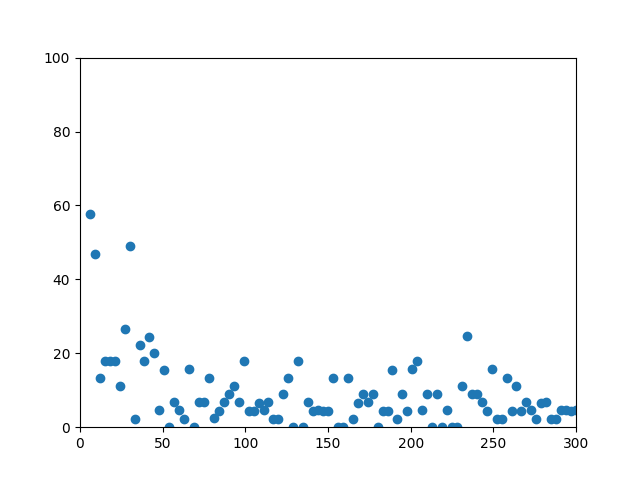
\includegraphics[width=8cm]{./tex_pic/figure.png}\\
\end{center}
上図より,鍵長は約50から値が変わらない,ということが読み取れる.よって鍵長は50文字以上である必要がある.また,上記「数学的アプローチ」と結果が近しいことから,実験の正確であることが証明できる.

\subsection{cubingmode以外の暗号利用モード}
暗号利用モードは他にも存在する.本節では暗号利用モードでも特に主流なCBCモード,CTRモード,CFBモードをcubing暗号で利用した際の安全性を考察する.

(※この節は保留にしています!!!!!!!!)

\section{課題}
\subsection{暗号文長}
cubing暗号は平文長が45Byteで暗号文長が54Byteである.cubing暗号を\(n\) (\(0 < n \leq 62^2\))ブロック暗号化すると,暗号文長は\(54n\)Byteになる.ここでcubingmodeを使用すると,mask処理によって1ブロック当たり52Byteのマスクが付与される.よって\(n\)ブロックの暗号化で出力されるデータ量は\(54n+52n=106n\)Byteである.これは平文長と比較して非常に多い.そこで,今後マスクは乱数であるシード値だけを暗号文に付加し,シード値から全てのマスクを生成できる多項式を選定し,cubingmodeのアルゴリズムに導入しようと考えている.

\subsection{暗号化に要する時間}
cubing暗号の暗号化に要する時間を測定した.測定には\url{https://github.com/xryuseix/cubing_cipher/tree/master/evalution/timecalc.cpp}を用いた.その結果,1秒間に約18MByteの暗号化が可能であることがわかった.しかし,同環境でOpenSSLによるAES(1024bit)の暗号化を行うと,1秒間に130MByteの暗号化ができた.今後の展開として,実装を少し工夫し,高速で暗号化を行えるようにしようと考えている.

\subsection{暗号文の順序}
ソースコードのアルゴリズムの出力は以下のようになっている.\\
\begin{screen}
  \begin{enumerate}
    \item block1とmask(1, 45)で使用したマスクの列
    \item block1のmask(46, 54)で使用したマスクの列
    \item block2とmask(1, 45)で使用したマスクの列
    \item block2のmask(46, 54)で使用したマスクの列 ...
  \end{enumerate}
\end{screen}
だが,以下のように出力した方が直感的である.\\
\begin{screen}
  \begin{enumerate}
    \item block1とmask(0, 45)で使用したマスクの列
    \item block2とmask(0, 45)で使用したマスクの列
    \item block1のmask(46, 54)で使用したマスクの列
    \item block2のmask(46, 54)で使用したマスクの列 ...
  \end{enumerate}
\end{screen}
これは,mask(46, 54)で使用したマスクの列に関してはどのmask(46, 54)で使用したマスクの列がどのブロックに適用されるのか判別できないと考えたからである.しかし,暗号文長をnとすると,先頭から\(\frac{54}{106}*n\)文字は暗号文ブロックである,という性質を利用すると正しく復号が可能である.ソースコードは今後は修正しようと考えている.

\section{関連研究}
本論文の先行研究としてまず“RUBIK'S CUBE” AS A TRANSPOSITION DEVICE\cite{Mitchell}という論文がある.この論文では同じくルービックキューブを用いた暗号について提案されている.暗号化の手順は以下の通りである.
\begin{enumerate}
  \item ルービックキューブの6つの面にそれぞれ1〜6まで数字を書き込む.ただし,1だけは面の左上のマスに書き込む.
  \item 面同士の入れ替えを行う.ただし,1が書かれている面に関しては入れ替えを行ってはならない.この時,並び替えの場合の総数は\(5!=120\)通り存在する.
  \item 各面に平文を8文字ずつ,数字が書かれていないマスに書き込む.
  \item ルービックキューブを回転させる.ただし,左上にある1の数字だけは回転させてはならない.
  \item スペースはランダム性のため,好きな数nullに置き換えても良い.
  \item 出来たルービックキューブの各面に書かれている数字の順に文字を取り出す.この時の文字が暗号文になる.
\end{enumerate}
この暗号はThe Rubik's Crypto-Cube: a Trans-Composite Cipher\cite{Trans-Composite Cipher}によって解読されている.Mitchell Cryptsystemsの弱点は主に二つある.一つ目はルービックキューブの角にある3マスは常に同じ位置関係にあること,二つ目は暗号文に使用される文字が平文の中にあることである.本論文のcubing暗号はこれらの弱点に対して対策を行った.\\
また,Scrambling algorithm for encryption of text using cube rotation artificial intelligence technique\cite{Scrambling algorithm}という論文でもルービックキューブを用いた暗号が使用されている.この論文ではルービックキューブの転置に対して人工知能を用いている.これにより暗号文は平文と比べ完全にスクランブルされると書かれている.しかし,暗号文の中に平文の文字が入った状態となってしまう他,改竄検知ができない.両者とも暗号アルゴリズムに脆弱性が存在したため,cubing暗号ではこれらに関して対策を行った.

\section{まとめ}

\subsection{本論文の内容}
本論文では自作の暗号cubing暗号についての定義とその安全性について述べた.ルービックキューブを用いた転置式暗号は既に開発されていたが,私はそれらの暗号を弱点を踏まえて解かれにくい暗号の作成を行った.解かれにくい暗号というのは,安全性が保証された条件下で様々な攻撃に対して無効である暗号である.

\subsection{推奨される鍵長に関して}
暗号の安全性が保証される鍵長に関しての検証も行った.検証は平文を転置した暗号文と元の平文との転置率を機械的に求める方法と数学的計算によって求める方法で二度行った.その結果,どちらも鍵長は50文字以上が好ましいとわかった.

\subsection{攻撃対策に関して}
本論文では主要な攻撃手法であるブルートフォース攻撃・頻度分析・選択平文攻撃・replay攻撃に関して,暗号の安全性の検証を行った.その結果,ブルートフォース攻撃に対しては最悪時間計算量が指数時間になるため,実用的ではないと判断できる.頻度分析に対しては暗号文がマスクされている上,たとえマスクが外されてもコンピュータ上で平文と予測した文字列が正しい平文であるという判定ができない.よって頻度分析も有用ではない.そして,選択平文攻撃に対してはマスク処理が施されており,マスクによって暗号文の各文字はランダムな値になる.最後に,replay攻撃に対しては,暗号文ブロックはシャッフルされるので,replay攻撃が成立する確率はブロック数を\(N\),すり替えたいブロック数を\(M\)とすると,\(\dfrac{1}{N^M}\)である.これは実用的ではない.\\
以上の結果から本暗号は以前から存在するルービックキューブによる転置式暗号の脆弱性を対策し,より安全な暗号の作成に成功した.

\section{謝辞}
本研究を進めるに当たり、サイボウズ・ラボ株式会社 緑川 志穂氏からは多大な助言を賜り,また丁寧に指導して下さいました。厚く感謝を申し上げます。また暗号の解読やアルゴリズム修正等を快く協力して頂いたセキュリティ・キャンプ2019集中開発コース標準ゼミのメンターの皆さま,及び様々な助言を頂きました受講生の皆さまにも感謝の意を表します.

\section{付録}
\subsection{1. 表示可能文字}
\begin{verbatim}
printable_table[] = {'0', '1', '2', '3', '4', '5', '6', '7', 
'8', '9', 'a', 'b', 'c', 'd', 'e', 'f', 'g', 'h', 'i', 'j', 'k', 
'l', 'm', 'n', 'o', 'p', 'q', 'r', 's', 't', 'u', 'v', 'w', 'x', 
'y', 'z', 'A', 'B', 'C', 'D', 'E', 'F', 'G', 'H', 'I', 'J', 'K', 
'L', 'M', 'N', 'O', 'P', 'Q', 'R', 'S', 'T', 'U', 'V', 'W', 'X', 
'Y', 'Z', '!', '"', '#', '$', '\%', '&', '\'', '(', ')', '*', '+', 
',', '-', '.', '/', ':', ';', '<', '=', '>', '?', '@', '[', '\\', 
']', '^', '_', '`', '{', '|', '}', '~', ' ', '\n', '\0', '\t'};
\end{verbatim}

\subsection{2. 62進数}
\begin{verbatim}
base62[]={'A', 'B', 'C', 'D', 'E', 'F', 'G', 'H', 'I', 'J', 'K', 
'L', 'M', 'N', 'O', 'P', 'Q', 'R', 'S', 'T', 'U', 'V', 'W', 'X', 
'Y', 'Z', 'a', 'b', 'c', 'd', 'e', 'f', 'g', 'h', 'i', 'j', 'k', 
'l', 'm', 'n', 'o', 'p', 'q', 'r', 's', 't', 'u', 'v', 'w', 'x', 
'y', 'z', '0', '1', '2', '3', '4', '5', '6', '7', '8', '9'}
\end{verbatim}
62進数の最初の数はAAであり,その次の数はABである.また,二桁で表すことのできる最も大きな数は99である.

\begin{flushleft}
\begin{thebibliography}{}

\bibitem{Mitchell} “RUBIK'S CUBE” AS A TRANSPOSITION DEVICE : https://www.tandfonline.com/doi/pdf/10.10\\80/0161-119291866928?needAccess=true

\bibitem{Trans-Composite Cipher}The Rubik's Crypto-Cube : a Trans-Composite Cipher : https://epublications.regis.edu/cgi/viewconte\\nt.cgi?article=1511\&context=theses

\bibitem{Scrambling algorithm}Scrambling algorithm for encryption of text using cube rotation artificial intelligence technique : https://pdfs.semanticscholar.org/1a63/be53b7\\ddc422107a9f4343eaa6cfe6732a70.pdf

\end{thebibliography}
\end{flushleft}

\end{document}
